\chapter[ĐẶT VẤN ĐỀ, PHÂN TÍCH YÊU CẦU VÀ KHÁM PHÁ DỮ LIỆU (EDA)]{ĐẶT VẤN ĐỀ, PHÂN TÍCH YÊU CẦU VÀ KHÁM PHÁ DỮ LIỆU (EDA)}

\section{Bối cảnh và mục tiêu của bài toán}

\subsection{Bối cảnh thực tiễn trong quản trị nguồn nhân lực}
Trong quản trị nguồn nhân lực hiện đại (\textit{Human Resource Management -- HRM}), tình trạng biến động nhân sự hay nghỉ việc tự nguyện (\textit{Employee Attrition / Turnover}) luôn là một trong những thách thức gây tốn kém nhất đối với doanh nghiệp. Khi một nhân viên có chuyên môn rời đi, tổ chức không chỉ chịu chi phí trực tiếp cho việc đăng tuyển, sàng lọc hồ sơ, phỏng vấn và đào tạo nhân sự thay thế, mà còn đối mặt với sự gián đoạn tiến độ dự án, sụt giảm năng suất đội ngũ và thất thoát tri thức tích lũy lâu năm.

Theo các nghiên cứu quản trị nhân sự, chi phí để thay thế một nhân viên kỹ thuật hoặc kinh doanh thường dao động từ $50\%$ đến $200\%$ mức lương hàng năm của vị trí đó. Trước đây, việc đánh giá nguy cơ nghỉ việc chủ yếu dựa vào cảm tính của người quản lý trực tiếp hoặc chỉ được ghi nhận thông qua buổi phỏng vấn thôi việc (\textit{Exit Interview}) --- tức là khi nhân viên đã đưa ra quyết định cuối cùng và doanh nghiệp không còn cơ hội can thiệp.

\subsection{Phát biểu bài toán học máy và mục tiêu nghiên cứu}
Bài toán \textbf{Đề tài 13: Dự đoán nhân viên có khả năng nghỉ việc} được phát biểu dưới dạng bài toán \textbf{phân loại nhị phân có giám sát (Supervised Binary Classification)} trên dữ liệu dạng bảng (\textit{Tabular Data}):
\begin{itemize}
    \item \textbf{Không gian đầu vào ($\mathbf{x}_i \in \mathbb{R}^d$)}: Mỗi nhân viên thứ $i$ được biểu diễn bởi một vector gồm các thuộc tính phản ánh nhân khẩu học (tuổi, giới tính, tình trạng hôn nhân, khoảng cách từ nhà đến công ty), đặc điểm công việc (phòng ban, vị trí, cấp bậc, tần suất đi công tác, làm thêm giờ), chế độ đãi ngộ (thu nhập hàng tháng, tỷ lệ tăng lương, quyền mua cổ phiếu), thâm niên công tác và các chỉ số khảo sát mức độ hài lòng.
    \item \textbf{Nhãn mục tiêu ($y_i \in \{0, 1\}$)}: Biến phân loại \textit{Attrition}, trong đó $y_i = 1$ (\textit{Yes}) tương ứng với nhân viên có khả năng nghỉ việc và $y_i = 0$ (\textit{No}) tương ứng với nhân viên tiếp tục gắn bó với doanh nghiệp.
    \item \textbf{Mục tiêu cốt lõi của bài tập lớn}:
    \begin{enumerate}
        \item Khám phá đặc trưng phân phối của bộ dữ liệu, phát hiện các yếu tố thúc đẩy nghỉ việc mạnh nhất và các vấn đề kỹ thuật của dữ liệu (mất cân bằng lớp, biến hằng số, biến định danh, ngoại lệ và đa cộng tuyến).
        \item Thiết kế và đối sánh hai luồng tiền xử lý dữ liệu (\textbf{Luồng A -- Cơ bản} và \textbf{Luồng B -- Cải tiến}) để trả lời câu hỏi: \textit{Thay đổi cách chuẩn bị dữ liệu và tạo đặc trưng mới có làm thay đổi hiệu quả của các thuật toán học máy hay không, và tại sao?}
        \item Huấn luyện, tinh chỉnh siêu tham số và so sánh các thuật toán đã học trong học phần (\textbf{K-Nearest Neighbors}, \textbf{Naive Bayes}, \textbf{Decision Tree}) cùng kỹ thuật mở rộng (\textbf{Random Forest}), từ đó đưa ra khuyến nghị ứng dụng thực tế cho phòng Nhân sự.
    \end{enumerate}
\end{itemize}

\section{Mô tả nguồn dữ liệu và cấu trúc thuộc tính}

\subsection{Nguồn gốc và kiểm tra chất lượng dữ liệu tổng quát}
Bộ dữ liệu sử dụng trong đề tài là \textbf{IBM HR Analytics Employee Attrition \& Performance} (tệp dữ liệu \textit{WA\_Fn-UseC\_-HR-Employee-Attrition.csv}), được chỉ định chính thức tại Mục 5.2 của Hướng dẫn thực hiện bài tập lớn học phần FIT4013. Qua quá trình kiểm tra tự động bằng mã nguồn khám phá dữ liệu:
\begin{itemize}
    \item \textbf{Số lượng mẫu ($N$)}: $1,470$ bản ghi (tương ứng với $1,470$ nhân viên).
    \item \textbf{Số lượng cột}: $35$ cột, bao gồm $34$ thuộc tính đầu vào và $1$ biến mục tiêu (\textit{Attrition}).
    \item \textbf{Dữ liệu khuyết thiếu (\textit{Missing values})}: Tất cả $35$ cột đều có đúng $1,470$ giá trị hợp lệ (số ô trống bằng $0$), không tồn tại giá trị khuyết hay chuỗi ký tự rỗng.
    \item \textbf{Dữ liệu trùng lặp (\textit{Duplicate rows})}: Không có bản ghi nào trùng lặp hoàn toàn (số dòng trùng lặp bằng $0$).
    \item \textbf{Kiểu dữ liệu}: Gồm $26$ thuộc tính kiểu số nguyên (\textit{int64}) và $9$ thuộc tính kiểu chuỗi phân loại (\textit{object / string}).
\end{itemize}

\subsection{Ý nghĩa các nhóm thuộc tính và phát hiện cột dư thừa}
Bảng~\ref{tab:mo-ta-thuoc-tinh} tổng hợp cấu trúc các nhóm thuộc tính trong bộ dữ liệu cùng vai trò của chúng trong mô hình học máy.

\begin{table}[H]
\caption{Phân nhóm và mô tả ý nghĩa 35 thuộc tính của bộ dữ liệu IBM HR Analytics}
\label{tab:mo-ta-thuoc-tinh}
\noindent
\begin{tabularx}{\textwidth}{|c|L{3.3cm}|L{4.4cm}|Y|}
\hline
\textbf{STT} & \textbf{Nhóm thuộc tính} & \textbf{Các cột đại diện} & \textbf{Đặc điểm và hướng xử lý} \\
\hline
1 & Biến mục tiêu (\textit{Target}) & \textit{Attrition} & Nhị phân: \textit{Yes} ($16.12\%$) và \textit{No} ($83.88\%$). Mã hóa thành $1 / 0$. \\
\hline
2 & Nhân khẩu học (\textit{Demographics}) & \textit{Age, Gender, MaritalStatus, DistanceFromHome, Education, EducationField} & Phản ánh độ tuổi ($18$--$60$), giới tính, hôn nhân và khoảng cách đi làm ($1$--$29$ dặm). \\
\hline
3 & Công việc và tổ chức (\textit{Job Profile}) & \textit{Department, JobRole, JobLevel, BusinessTravel, OverTime} & Phản ánh vị trí ($9$ vai trò), phòng ban ($3$ phòng ban), tần suất công tác và làm thêm giờ. \\
\hline
4 & Lương và đãi ngộ (\textit{Compensation}) & \textit{MonthlyIncome, PercentSalaryHike, StockOptionLevel, DailyRate, HourlyRate, MonthlyRate} & \textit{MonthlyIncome} có tương quan mạnh với nghỉ việc; riêng $3$ cột \textit{Rate} là nhiễu ngẫu nhiên. \\
\hline
5 & Khảo sát hài lòng (\textit{Survey Scores}) & \textit{JobSatisfaction, EnvironmentSatisfaction, RelationshipSatisfaction, WorkLifeBalance, JobInvolvement} & Thang đo thứ bậc từ $1$ (Thấp) đến $4$ (Rất cao) phản ánh cảm nhận về môi trường làm việc. \\
\hline
6 & Thâm niên và kinh nghiệm (\textit{Tenure}) & \textit{TotalWorkingYears, YearsAtCompany, YearsInCurrentRole, YearsSinceLastPromotion, YearsWithCurrManager, NumCompaniesWorked} & Đo lường bề dày kinh nghiệm, sự ổn định tại công ty và tốc độ thăng tiến. \\
\hline
7 & Cột hằng số và định danh (\textit{Redundant/ID}) & \textit{EmployeeCount, Over18, StandardHours, EmployeeNumber} & Không mang thông tin phân lớp hoặc gây học vẹt $\rightarrow$ \textbf{Loại bỏ ở cả Luồng A và B}. \\
\hline
\end{tabularx}
\Nguon{Nhóm thực hiện tổng hợp từ bộ dữ liệu IBM HR Analytics}
\end{table}

Cụ thể, qua phân tích số lượng giá trị phân biệt trên từng cột, nhóm phát hiện $4$ cột bắt buộc phải loại bỏ trước khi đưa vào mô hình:
\begin{enumerate}
    \item \textit{EmployeeCount}: Mọi dòng đều có giá trị bằng $1$ (số giá trị phân biệt bằng $1$, phương sai bằng $0$).
    \item \textit{Over18}: Mọi nhân viên đều trên $18$ tuổi, nhận giá trị hằng số \textit{'Y'} (số giá trị phân biệt bằng $1$).
    \item \textit{StandardHours}: Mọi dòng đều có số giờ tiêu chuẩn bằng $80$ (số giá trị phân biệt bằng $1$).
    \item \textit{EmployeeNumber}: Mã định danh duy nhất của từng nhân viên ($1,470$ giá trị khác nhau, trải từ $1$ đến $2,068$). Nếu giữ lại cột này, Cây quyết định có thể cắt nhánh theo số thứ tự bản ghi, gây quá khớp (\textit{overfitting}) nghiêm trọng.
\end{enumerate}

\section{Khám phá và phân tích dữ liệu chuyên sâu (EDA)}

\subsection{Phân tích phân phối biến mục tiêu và bài toán mất cân bằng lớp}
Hình~\ref{fig:target_dist} biểu diễn phân phối số lượng và tỷ lệ phần trăm của biến mục tiêu \textit{Attrition} trên toàn bộ $1,470$ nhân viên.

\begin{figure}[H]
    \centering
    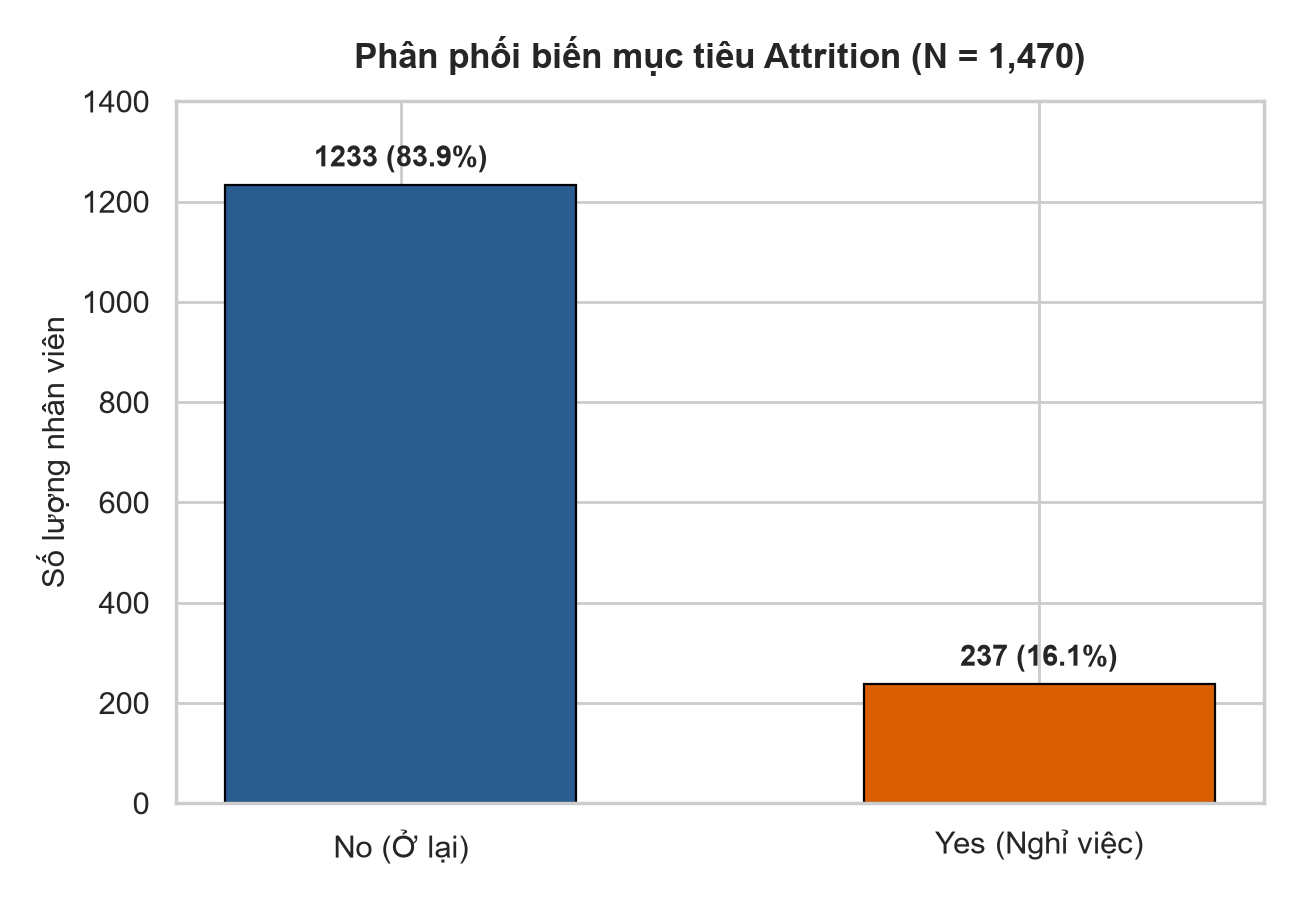
\includegraphics[width=0.68\textwidth]{images/fig1_target_distribution.png}
    \caption{Phân phối biến mục tiêu Attrition trên tập dữ liệu ($N = 1,470$)}
    \label{fig:target_dist}
    \Nguon{Nhóm thực hiện trích xuất từ dữ liệu thực nghiệm}
\end{figure}

Từ Hình~\ref{fig:target_dist}, ta thấy rõ cấu trúc \textbf{mất cân bằng lớp (\textit{Class Imbalance})}:
\begin{itemize}
    \item Nhóm \textbf{\textit{No} (Ở lại)}: gồm $1,233$ nhân viên, chiếm \textbf{83.88\%}.
    \item Nhóm \textbf{\textit{Yes} (Nghỉ việc)}: gồm $237$ nhân viên, chiếm \textbf{16.12\%}.
\end{itemize}
Tỷ lệ giữa lớp đa số và lớp thiểu số là $1233 / 237 \approx \mathbf{5.20 : 1}$. Đặc điểm này dẫn đến hai hệ quả quan trọng cho thiết kế quy trình học máy của nhóm:
\begin{enumerate}
    \item \textbf{Về phương pháp chia dữ liệu}: Bắt buộc phải sử dụng kỹ thuật chia phân tầng (\textit{Stratified Train/Test Split} và \textit{StratifiedKFold}) để đảm bảo tỷ lệ $16.12\%$ mẫu nghỉ việc được giữ nguyên đồng đều trên cả tập huấn luyện và tập kiểm thử.
    \item \textbf{Về độ đo đánh giá (\textit{Evaluation Metrics})}: Một bộ phân loại tầm thường (\textit{Dummy Classifier}) luôn dự đoán mọi nhân viên đều ``Ở lại (\textit{No})'' vẫn sẽ đạt độ chính xác tổng thể $\text{Accuracy} = 83.88\%$, nhưng lại có $\text{Recall} = 0\%$ và $\text{F1-score} = 0\%$ đối với lớp nghỉ việc. Vì vậy, theo đúng yêu cầu của học phần, nhóm không đánh giá mô hình chỉ dựa trên \textit{Accuracy} mà đặt trọng tâm vào \textbf{F1-score}, \textbf{Recall}, \textbf{Precision}, \textbf{Confusion Matrix} và \textbf{ROC-AUC}.
\end{enumerate}

\subsection{Phân tích các đặc trưng số, ngoại lệ (Outliers) và hiện tượng đa cộng tuyến}
Bảng~\ref{tab:thong-ke-mo-ta} trình bày các chỉ số thống kê mô tả của $10$ đặc trưng số tiêu biểu. Tiếp theo, Hình~\ref{fig:boxplots} trực quan hóa phân phối và các điểm ngoại lệ (\textit{outliers}) bằng biểu đồ Boxplot giữa hai lớp \textit{Attrition = No} và \textit{Attrition = Yes}.

\begin{table}[H]
\caption{Thống kê mô tả các đặc trưng số tiêu biểu ($N = 1,470$)}
\label{tab:thong-ke-mo-ta}
\noindent
\begin{tabularx}{\textwidth}{|Y|r|r|r|r|r|r|}
\hline
\textbf{Tên đặc trưng} & \textbf{Mean} & \textbf{Std} & \textbf{Min} & \textbf{Q25} & \textbf{Median} & \textbf{Max} \\
\hline
\textit{Age} (Tuổi) & 36.92 & 9.14 & 18.0 & 30.0 & 36.0 & 60.0 \\
\hline
\textit{MonthlyIncome} (USD) & 6,502.93 & 4,707.96 & 1,009.0 & 2,911.0 & 4,919.0 & 19,999.0 \\
\hline
\textit{TotalWorkingYears} (Năm) & 11.28 & 7.78 & 0.0 & 6.0 & 10.0 & 40.0 \\
\hline
\textit{YearsAtCompany} (Năm) & 7.01 & 6.13 & 0.0 & 3.0 & 5.0 & 40.0 \\
\hline
\textit{YearsInCurrentRole} (Năm) & 4.23 & 3.62 & 0.0 & 2.0 & 3.0 & 18.0 \\
\hline
\textit{YearsSinceLastPromotion} & 2.19 & 3.22 & 0.0 & 0.0 & 1.0 & 15.0 \\
\hline
\textit{DistanceFromHome} (Dặm) & 9.19 & 8.11 & 1.0 & 2.0 & 7.0 & 29.0 \\
\hline
\textit{NumCompaniesWorked} & 2.69 & 2.50 & 0.0 & 1.0 & 2.0 & 9.0 \\
\hline
\textit{PercentSalaryHike} (\%) & 15.21 & 3.66 & 11.0 & 12.0 & 14.0 & 25.0 \\
\hline
\textit{DailyRate} & 802.49 & 403.51 & 102.0 & 465.0 & 802.0 & 1,499.0 \\
\hline
\end{tabularx}
\Nguon{Nhóm thực hiện tính toán từ tập dữ liệu}
\end{table}

\begin{figure}[H]
    \centering
    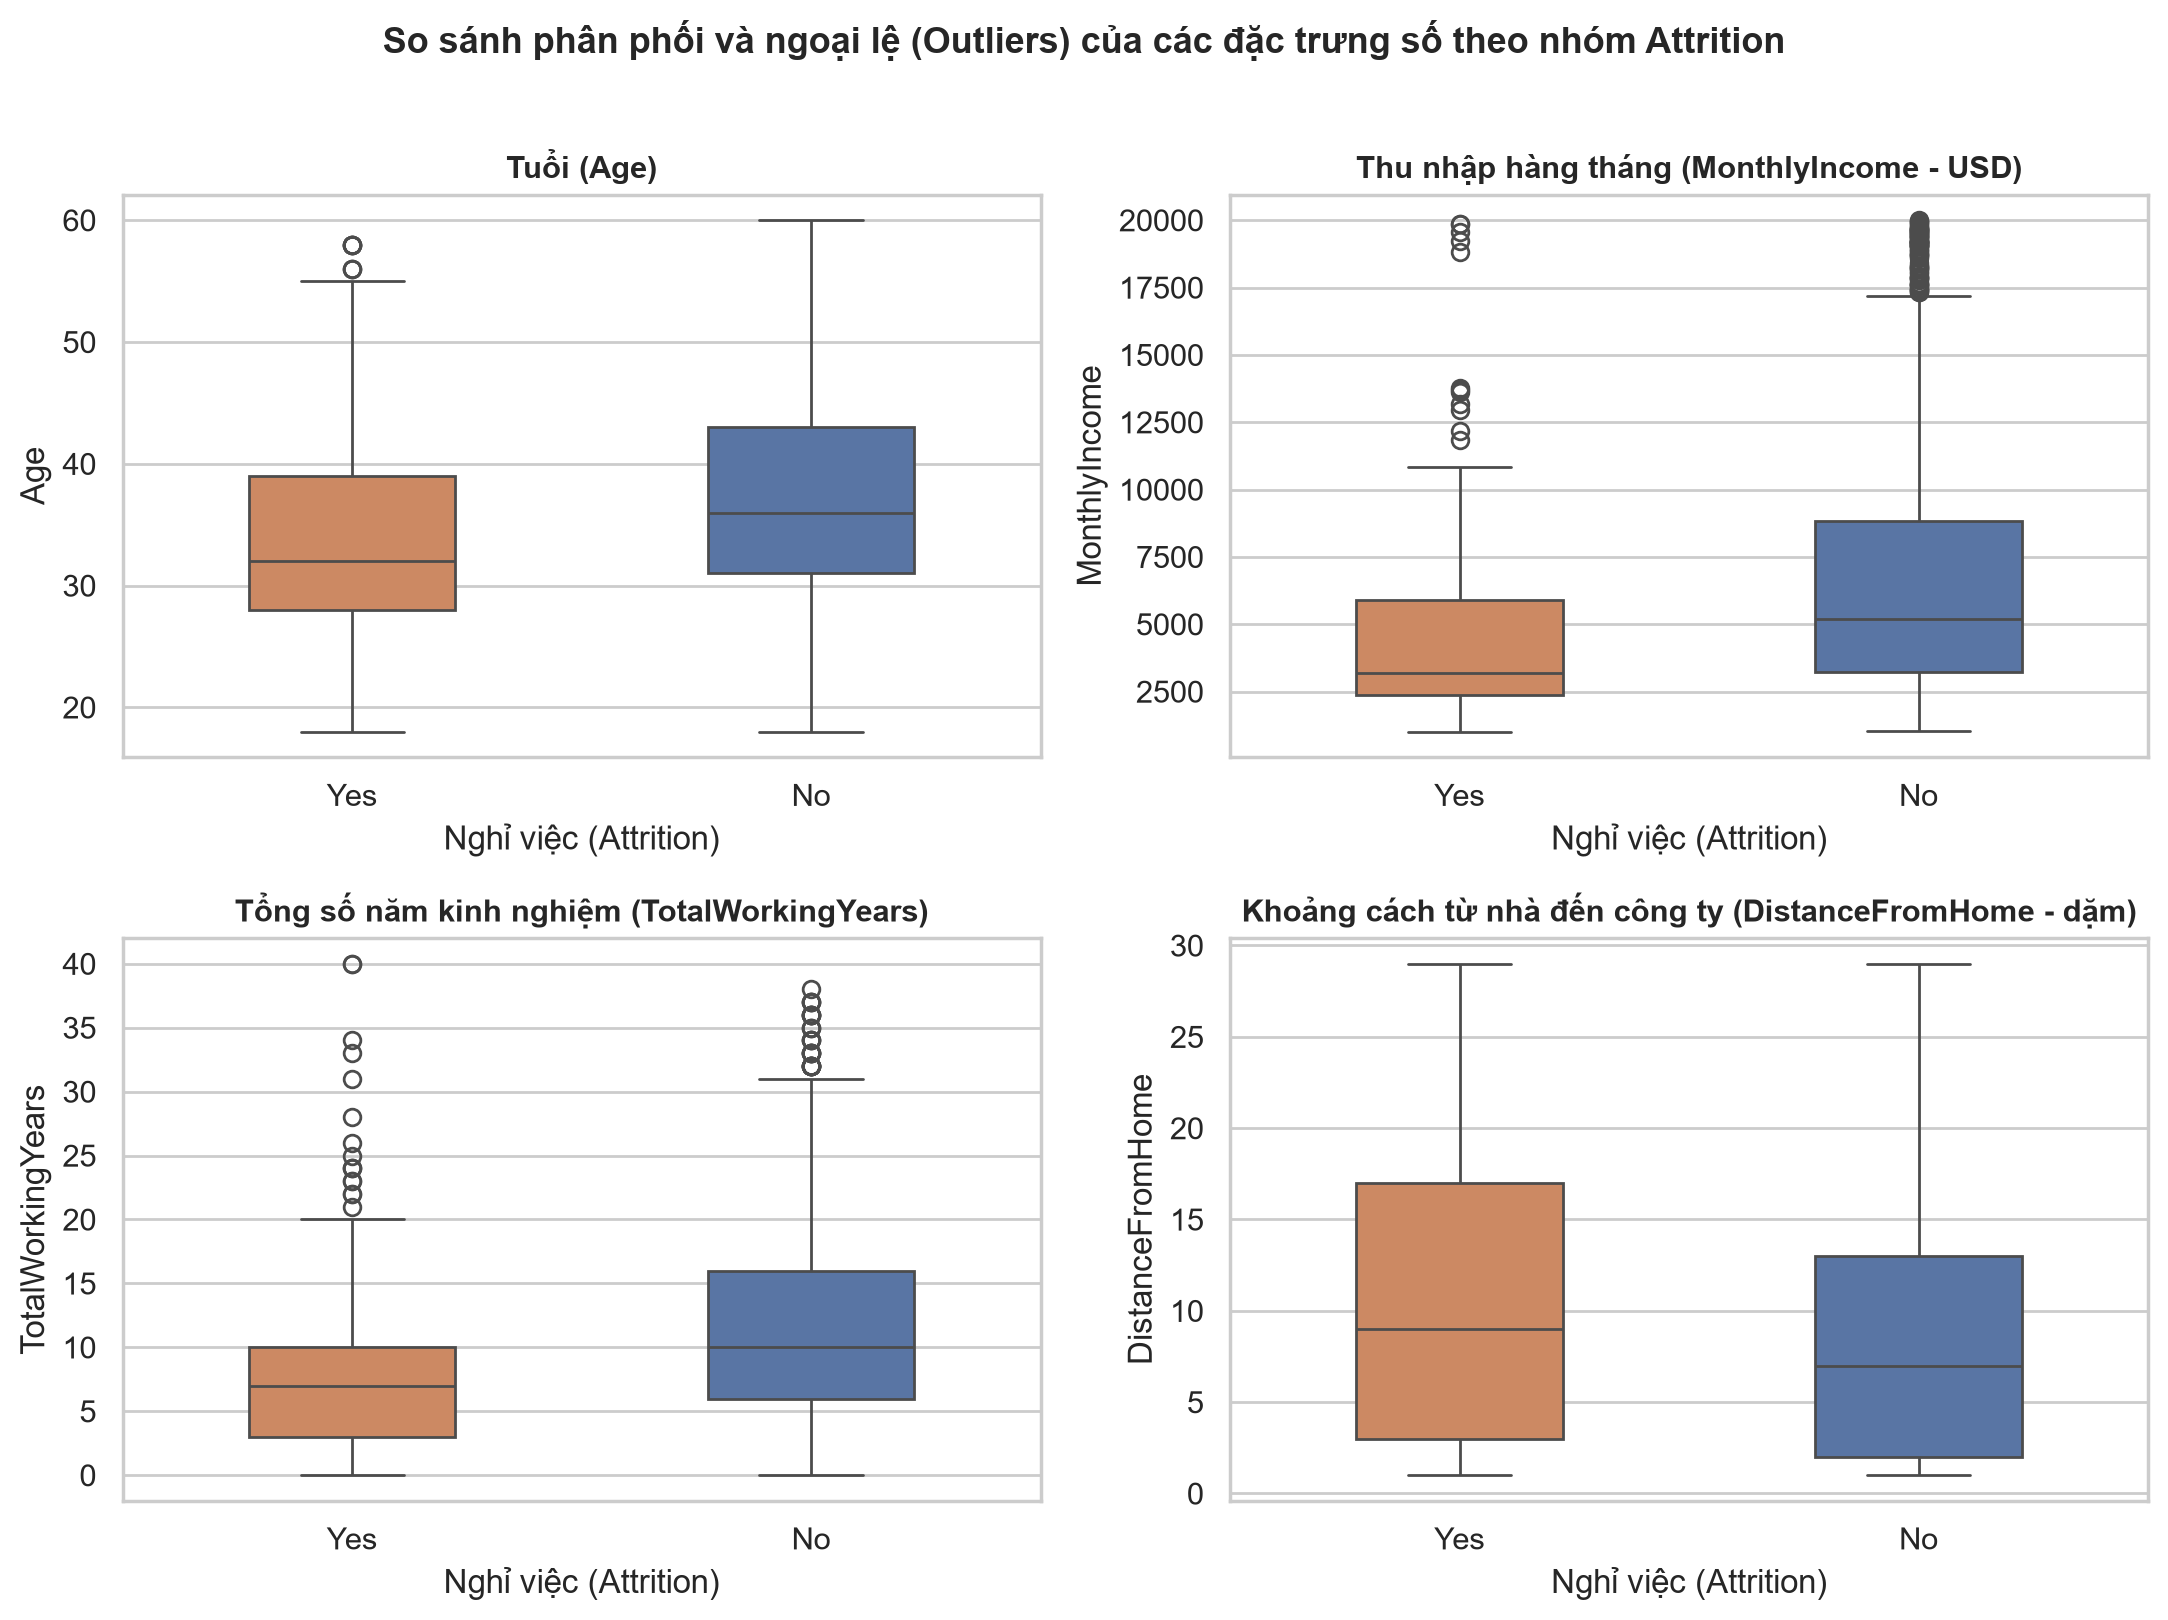
\includegraphics[width=0.95\textwidth]{images/fig2_numerical_boxplots.png}
    \caption{Biểu đồ Boxplot so sánh phân phối và ngoại lệ của các đặc trưng số theo nhóm Attrition}
    \label{fig:boxplots}
    \Nguon{Nhóm thực hiện trích xuất từ dữ liệu thực nghiệm}
\end{figure}

Để kiểm tra mối quan hệ tuyến tính giữa các biến số, Hình~\ref{fig:corr_heatmap} trình bày ma trận tương quan Pearson của các biến số chính và biến mục tiêu đã mã hóa nhị phân \textit{Attrition\_num}.

\begin{figure}[H]
    \centering
    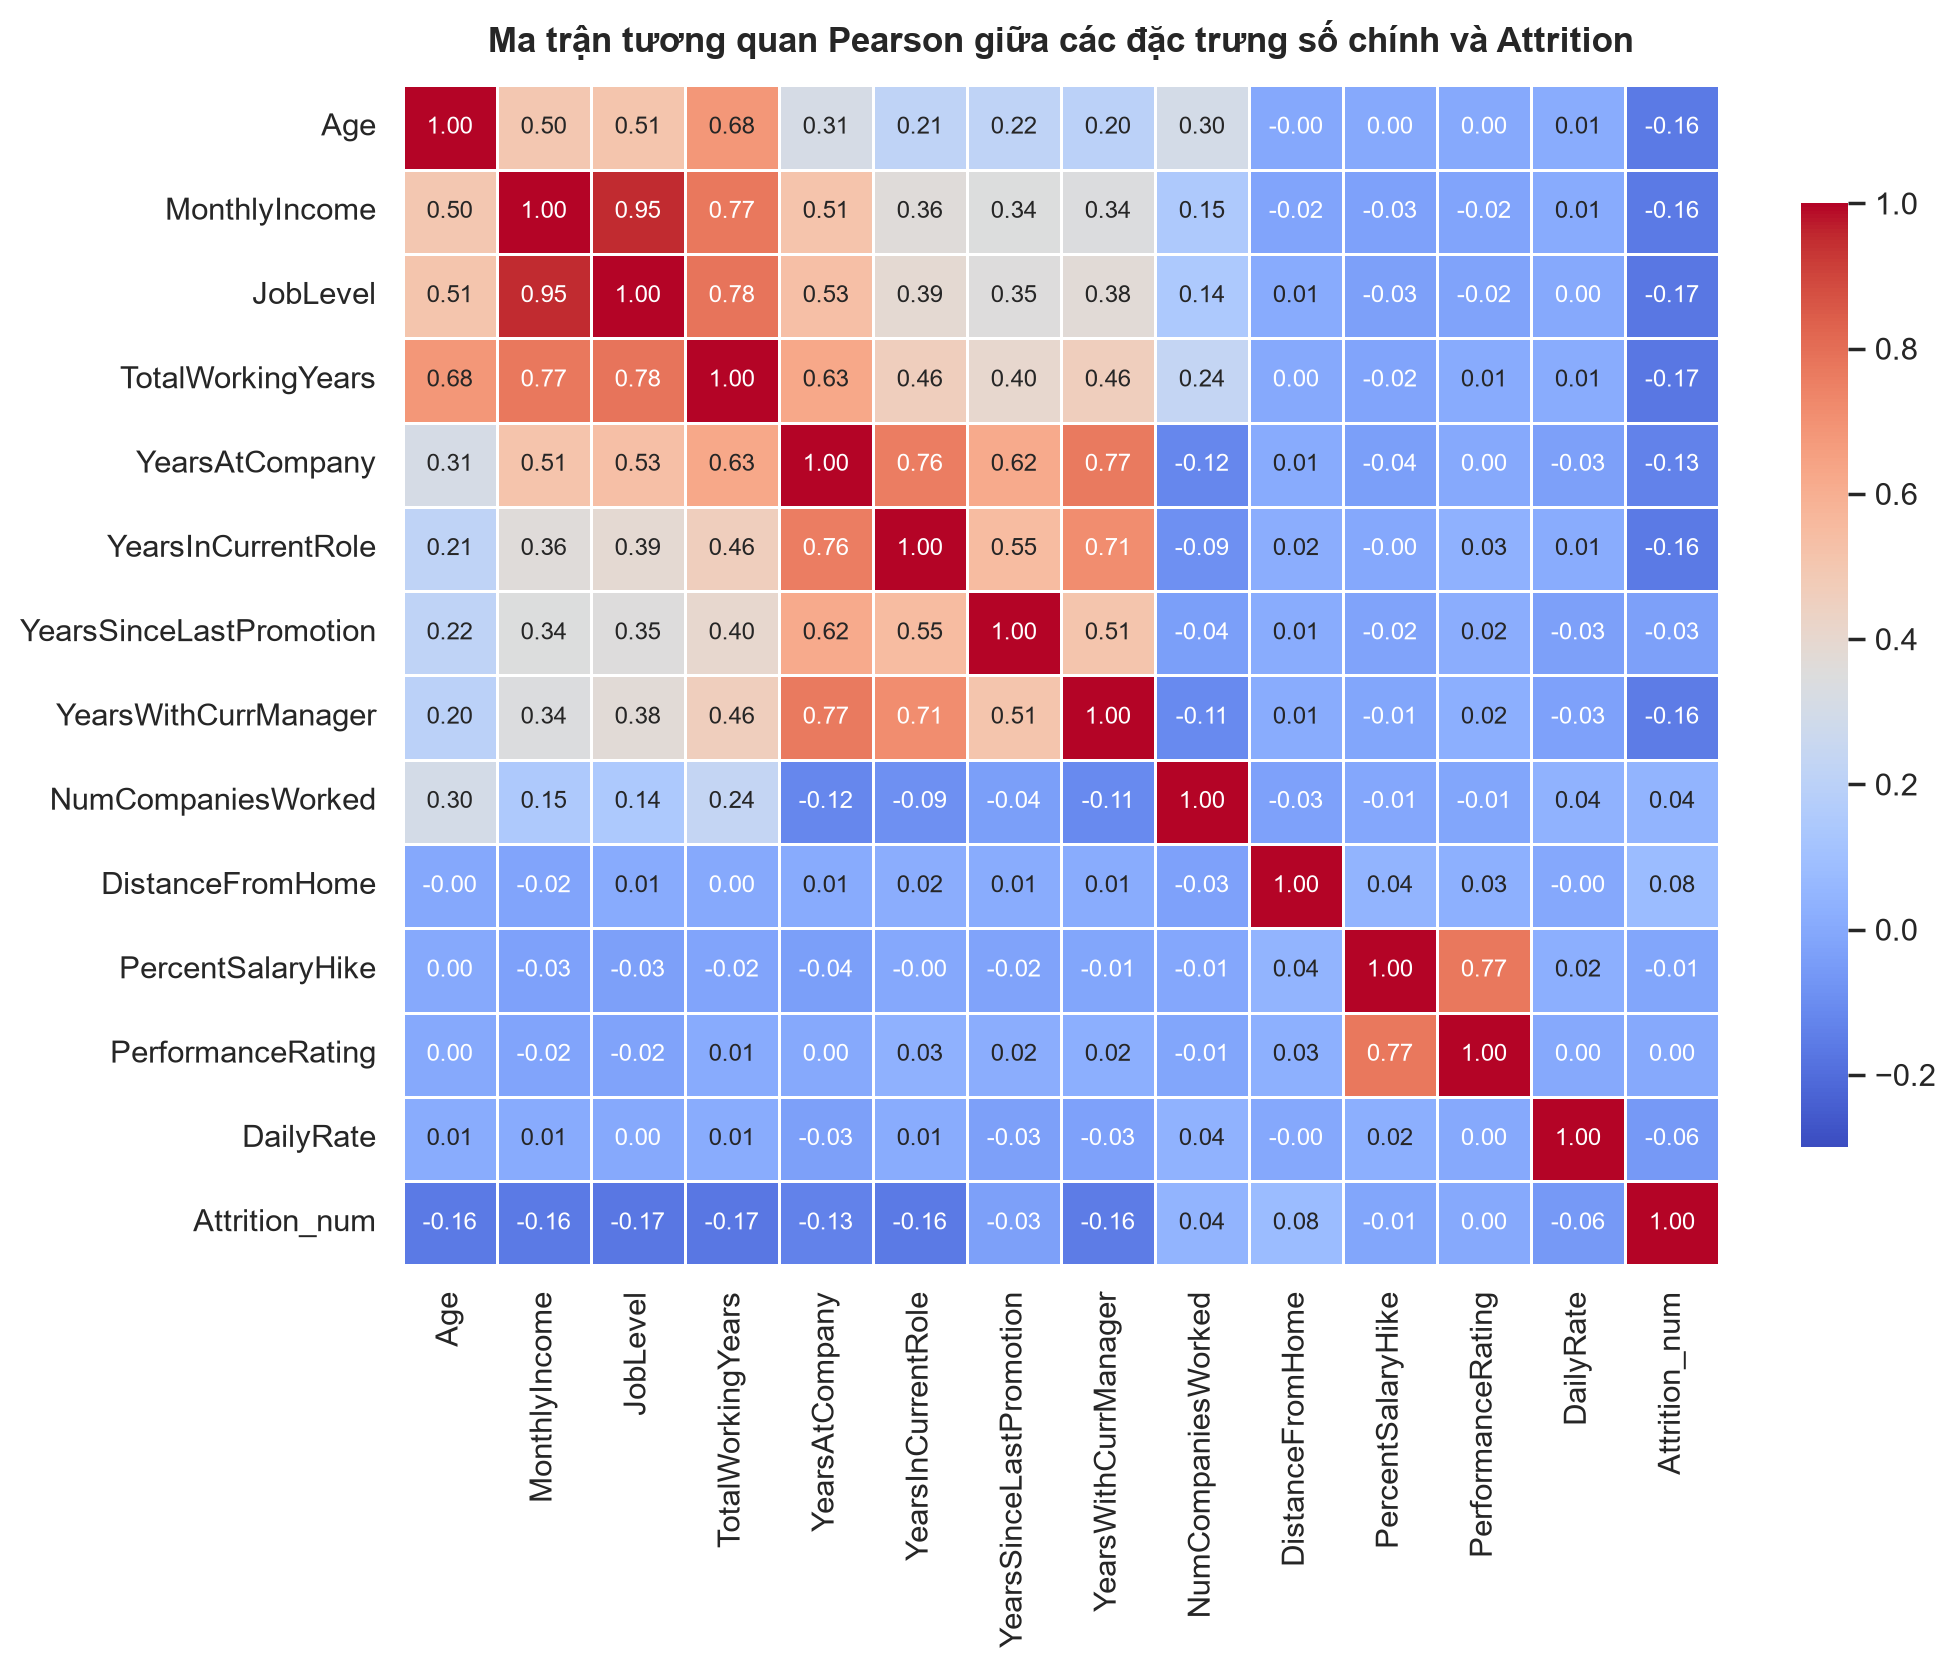
\includegraphics[width=0.88\textwidth]{images/fig4_correlation_heatmap.png}
    \caption{Ma trận tương quan Pearson giữa các đặc trưng số và biến mục tiêu Attrition}
    \label{fig:corr_heatmap}
    \Nguon{Nhóm thực hiện trích xuất từ dữ liệu thực nghiệm}
\end{figure}

Qua đối chiếu Bảng~\ref{tab:thong-ke-mo-ta}, Hình~\ref{fig:boxplots} và Hình~\ref{fig:corr_heatmap}, nhóm rút ra ba nhận định kỹ thuật cốt lõi phục vụ thiết kế Luồng B:
\begin{enumerate}
    \item \textbf{Sự khác biệt rõ rệt về thu nhập, tuổi và thâm niên giữa hai lớp}: Nhóm nhân viên nghỉ việc (\textit{Yes}) có trung vị thu nhập hàng tháng thấp hơn đáng kể so với nhóm ở lại ($\approx 3,202$ USD so với $5,204$ USD; $r = -0.1598$), tổng số năm kinh nghiệm ít hơn ($r = -0.1711$), số năm ở vị trí hiện tại thấp hơn ($r = -0.1605$), tuổi đời trẻ hơn ($r = -0.1592$) và khoảng cách từ nhà đến nơi làm việc xa hơn ($r = +0.0779$).
    \item \textbf{Phân phối lệch phải mạnh và nhiều ngoại lệ (\textit{Outliers})}: Các biến \textit{MonthlyIncome} (trung bình $6,503$ USD nhưng trung vị chỉ $4,919$ USD, cực đại lên tới $19,999$ USD), \textit{TotalWorkingYears} và \textit{YearsAtCompany} có đuôi phân phối lệch phải dài với nhiều điểm ngoại lệ ở nhóm quản lý cấp cao. Nếu chỉ dùng bộ chuẩn hóa \textit{StandardScaler} (chuẩn hóa theo trung bình và độ lệch chuẩn), các ngoại lệ này sẽ kéo dãn thang đo, làm co cụm các nhân viên lương thấp lại gần nhau. Do đó, sử dụng \textbf{\textit{RobustScaler}} (chuẩn hóa theo trung vị và khoảng tứ phân vị IQR) ở Luồng B là giải pháp hợp lý hơn.
    \item \textbf{Phát hiện biến nhiễu ngẫu nhiên và đa cộng tuyến mạnh}:
    \begin{itemize}
        \item Ba biến \textit{DailyRate} ($r = -0.0567$), \textit{HourlyRate} ($r = -0.0068$) và \textit{MonthlyRate} ($r = +0.0152$) có phân phối đều ngẫu nhiên và hoàn toàn không liên quan tới \textit{MonthlyIncome} ($r \approx 0$). Giữ lại $3$ cột này chỉ làm tăng nhiễu khoảng cách Euclidean trong K-NN.
        \item Biến \textit{JobLevel} tương quan gần như tuyệt đối với \textit{MonthlyIncome} ($r = \mathbf{0.95}$); biến \textit{PercentSalaryHike} tương quan chặt với \textit{PerformanceRating} ($r = \mathbf{0.77}$); các biến thâm niên \textit{YearsAtCompany}, \textit{YearsInCurrentRole}, \textit{YearsWithCurrManager} có tương quan lẫn nhau từ $0.71$ đến $0.77$. Hiện tượng \textbf{đa cộng tuyến (\textit{Multicollinearity})} này vi phạm trực tiếp giả định độc lập có điều kiện của thuật toán Naive Bayes, làm nhân đôi trọng số của cùng một nguồn thông tin và gây sai lệch xác suất dự đoán.
    \end{itemize}
\end{enumerate}

\subsection{Phân tích các đặc trưng phân loại và hình thành giả thuyết kỹ thuật đặc trưng}
Hình~\ref{fig:cat_rates} trực quan hóa tỷ lệ nghỉ việc (\%) trên từng giá trị của $4$ thuộc tính phân loại quan trọng nhất: \textit{OverTime}, \textit{MaritalStatus}, \textit{BusinessTravel} và \textit{JobRole}.

\begin{figure}[H]
    \centering
    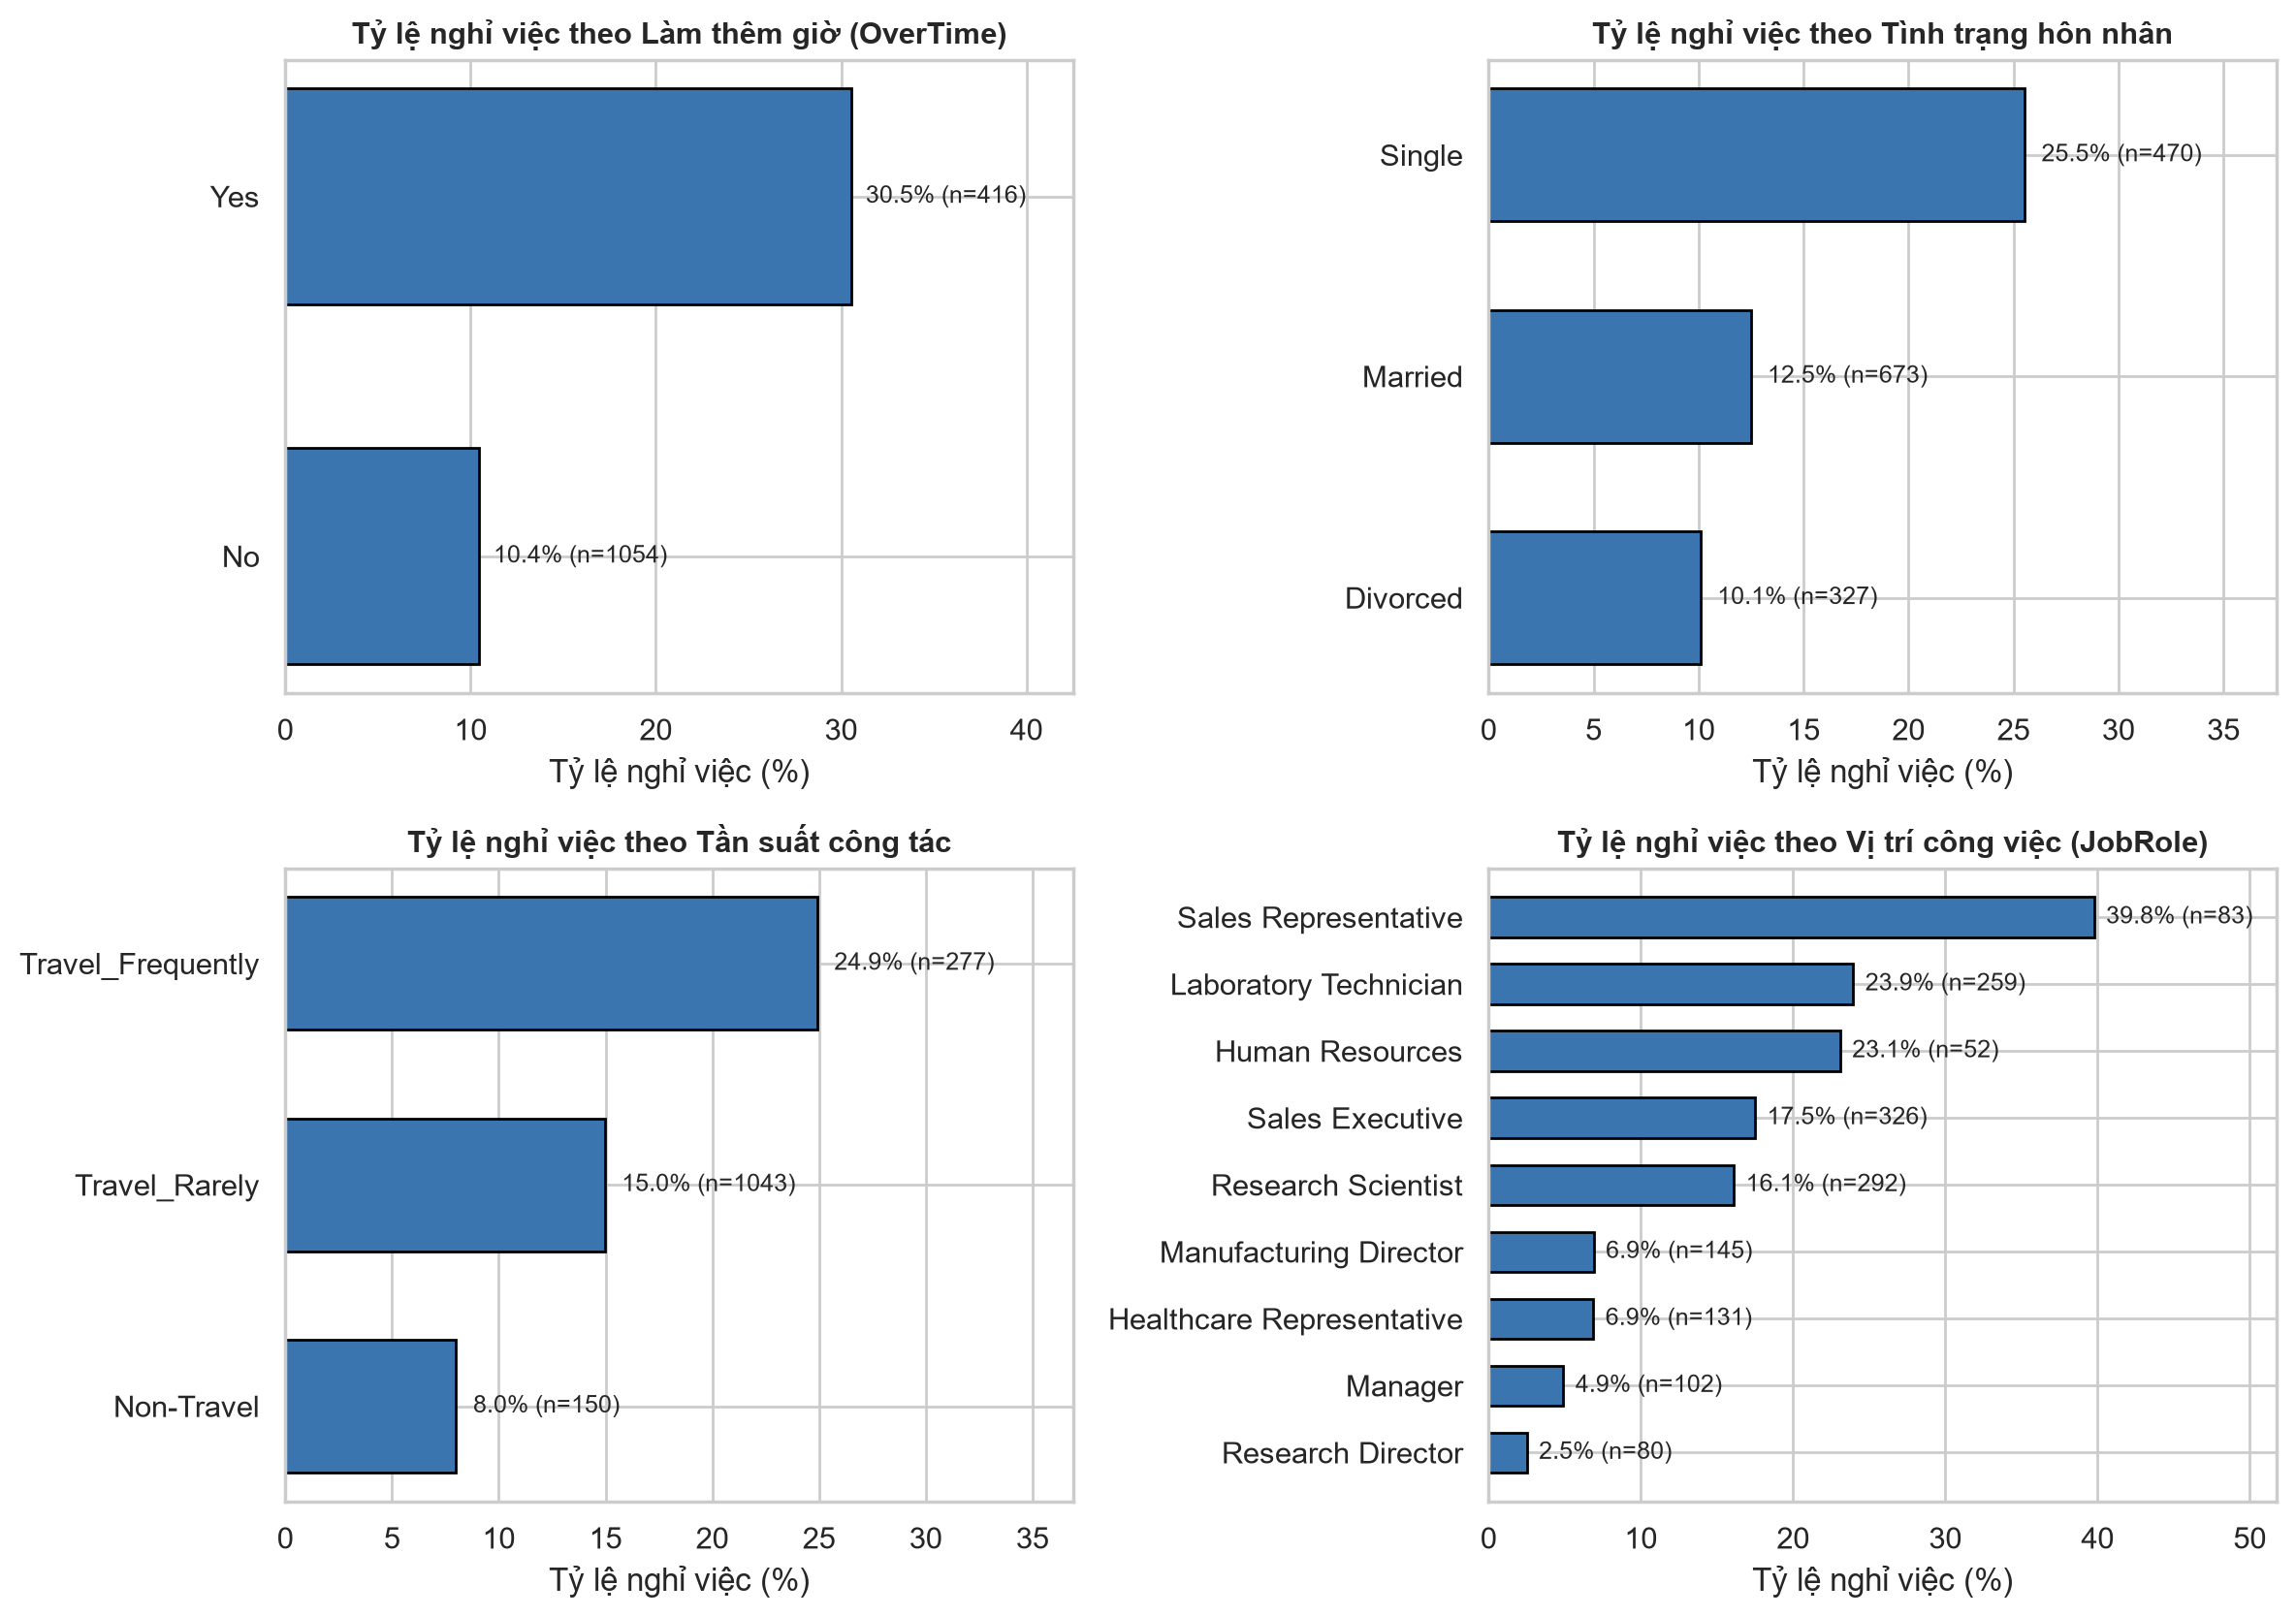
\includegraphics[width=0.96\textwidth]{images/fig3_categorical_rates.png}
    \caption{Tỷ lệ nghỉ việc (\%) theo 4 đặc trưng phân loại quan trọng}
    \label{fig:cat_rates}
    \Nguon{Nhóm thực hiện trích xuất từ dữ liệu thực nghiệm}
\end{figure}

Phân tích thống kê từ Hình~\ref{fig:cat_rates} cho thấy các quy luật nghiệp vụ rất rõ nét:
\begin{itemize}
    \item \textbf{Tác động đột biến của Làm thêm giờ (\textit{OverTime})}: Trong số $416$ nhân viên phải làm thêm giờ (\textit{OverTime = Yes}), có tới $127$ người nghỉ việc (\textbf{30.53\%}), cao gấp gần \textbf{3 lần} so với nhóm không làm thêm giờ (\textbf{10.44\%}, $110/1,054$ người). Đây là biến đơn lẻ có sức phân tách mạnh nhất trong toàn bộ tập dữ liệu.
    \item \textbf{Tình trạng hôn nhân (\textit{MaritalStatus})}: Nhân viên độc thân (\textit{Single}) có tỷ lệ nghỉ việc lên tới \textbf{25.53\%} ($120/470$ người), cao hơn gấp đôi so với nhân viên đã kết hôn (\textit{Married}: \textbf{12.48\%}) và nhân viên đã ly hôn (\textit{Divorced}: \textbf{10.09\%}).
    \item \textbf{Tần suất đi công tác (\textit{BusinessTravel})}: Nhóm phải đi công tác thường xuyên (\textit{Travel\_Frequently}) có tỷ lệ nghỉ việc \textbf{24.91\%}, cao gấp $3$ lần nhóm không phải đi công tác (\textit{Non-Travel}: \textbf{8.00\%}).
    \item \textbf{Vị trí công việc (\textit{JobRole})}: Vị trí nhân viên kinh doanh (\textit{Sales Representative}) có tỷ lệ biến động nhân sự báo động ở mức \textbf{39.76\%} ($33/83$ người), tiếp theo là kỹ thuật viên phòng thí nghiệm (\textit{Laboratory Technician}: \textbf{23.94\%}) và chuyên viên nhân sự (\textit{Human Resources}: \textbf{23.08\%}). Ngược lại, các cấp quản lý như \textit{Research Director} ($2.50\%$) và \textit{Manager} ($4.90\%$) có tỷ lệ nghỉ việc rất thấp.
\end{itemize}

\textbf{Hình thành giả thuyết cho Luồng B}: Nghỉ việc hiếm khi chỉ do một yếu tố đơn lẻ mà thường là kết quả cộng hưởng của nhiều áp lực đồng thời --- chẳng hạn: \textit{nhân viên trẻ/độc thân phải làm thêm giờ liên tục}, \textit{làm thêm giờ kèm theo quãng đường đi làm xa}, hoặc \textit{mức thu nhập thấp không tương xứng với số năm kinh nghiệm và nhiều năm chưa được thăng chức}. Việc tổng hợp các mối quan hệ tương tác này thành các đặc trưng mới sẽ giúp mô hình tuyến tính/xác suất và cây quyết định độ sâu thấp nắm bắt quy luật tốt hơn nhiều so với các cột thô rời rạc.
